%!TEX root = ../tesis_mbc.tex

\chapter{Resultados}

Los algoritmos presentados en este trabajo fueron implementados en el lenguaje para cómputo estadístico R y fueron probados con un conjunto de películas calificadas de \textit{MovieLens}, una página que ofrece recomendaciones de películas, los cuales están disponibles al público. \textit{MovieLens} es un proyecto de \textit{GroupLens}, un equipo de investigación de la Universidad de Minnesota orientado al cómputo social.

\subsection{Análisis exploratorio de datos}

\subsubsection{\textit{MovieLens}}

El conjunto de datos de \textit{MovieLens} consiste en \numprint{20000263} calificaciones de \numprint{26744} películas hechas por \numprint{138493} usuarios. Todos los usuarios habían calificado al menos 20 películas. Las calificaciones están en una escala de $0.5$ a $5$, con intervalos de medio punto, es decir, se puede poner $0.5, 1, \hdots, 4.5, 5$ como calificación. La distribución de las calificaciones se puede ver en la figura \ref{fig:ML_frec_calificaciones}.

\begin{figure}[!h]
	\centering
 	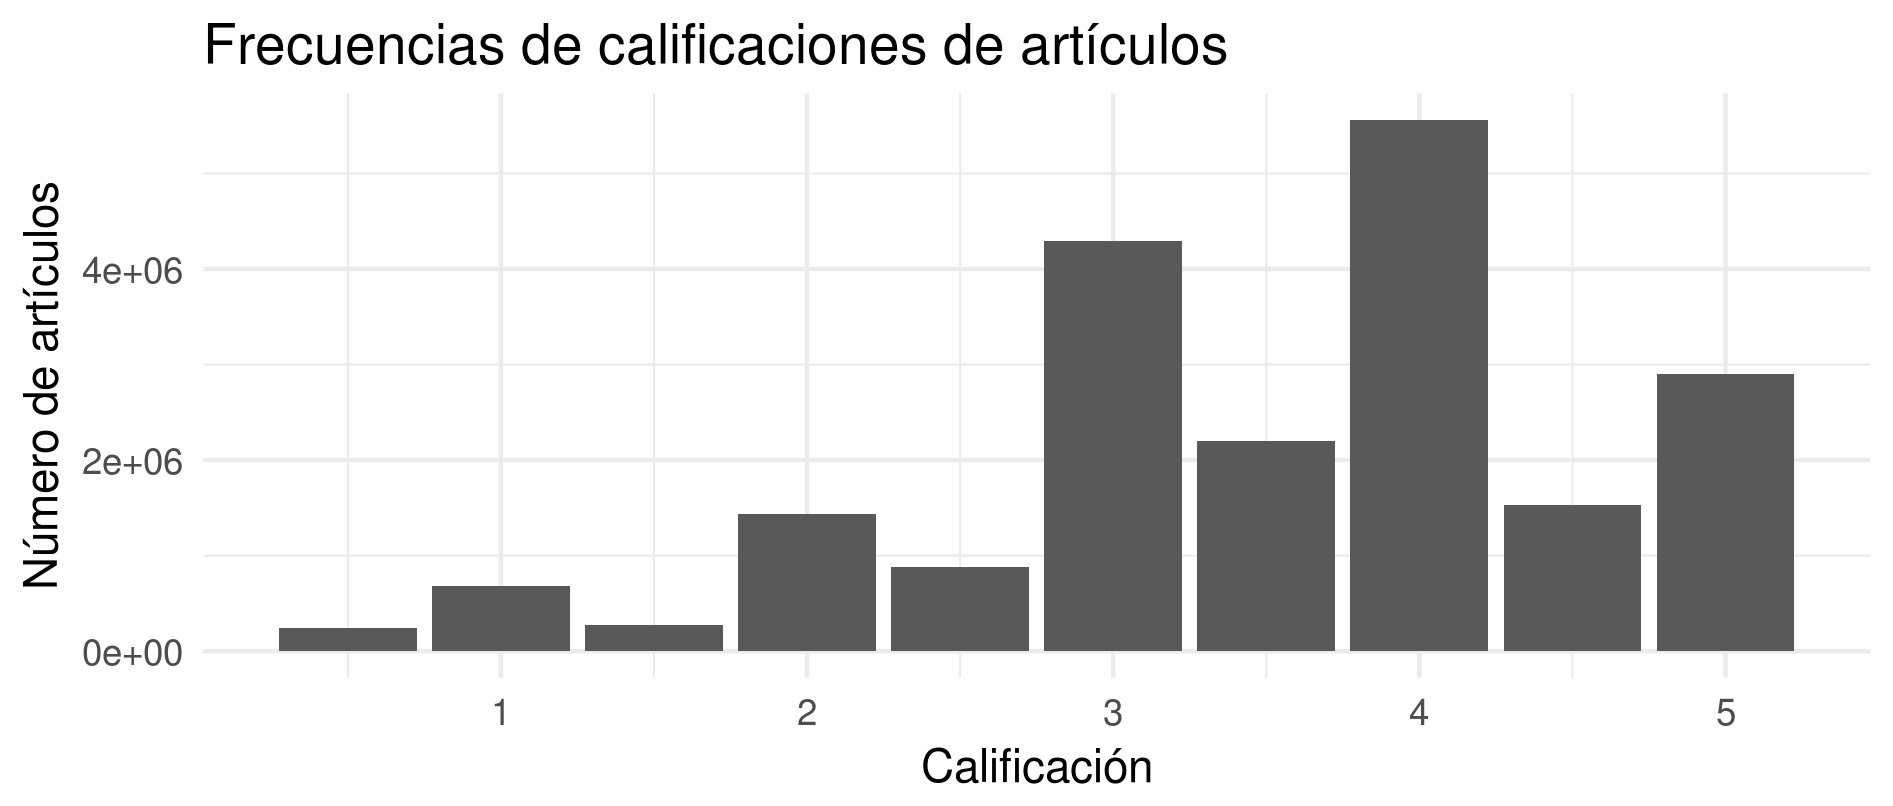
\includegraphics[width=0.9\textwidth]{frecuencia_calificaciones_MovieLens.png}
 	\caption{Frecuencia de calificaciones del conjunto de datos \textit{MovieLens}.}
 	\label{fig:ML_frec_calificaciones}
\end{figure}




